\chapter{الگوریتم‌های رشته}

این فصل به الگوریتم‌های کارآمد برای پردازش رشته می‌پردازد.
بسیاری از مسائل رشته به سادگی در زمان $O(n^2)$ حل می‌شوند، اما چالش اصلی یافتن الگوریتم‌هایی با زمان اجرای $O(n)$ یا $O(n \log n)$ است.

\index{pattern matching@تطابق الگو}

برای نمونه، یک مسئله بنیادین پردازش رشته مسئله \key{تطابق الگو} است:
به ازای یک رشته به طول $n$ و یک الگو به طول $m$، هدف یافتن تمام رخدادهای الگو در رشته است.
مثلاً، الگوی \texttt{ABC} دو بار در رشته \texttt{ABABCBABC} ظاهر می‌شود.

مسئله تطابق الگو به سادگی با یک الگوریتم جستجوی کامل (brute force) در زمان $O(nm)$ حل می‌شود؛ الگوریتمی که تمام جایگاه‌های ممکن رخداد الگو را بررسی می‌کند.
با این حال، در این فصل خواهیم دید الگوریتم‌های کارآمدتری وجود دارند که تنها به زمان $O(n+m)$ نیاز دارند.

\index{string@رشته}

\section{اصطلاحات رشته}

\index{alphabet@الفبا}

در سراسر این فصل، فرض می‌شود اندیس‌گذاری رشته‌ها از صفر آغاز می‌شود.
بنابراین، رشته \texttt{s} به طول $n$ شامل نویسه‌های
$\texttt{s}[0],\texttt{s}[1],\ldots,\texttt{s}[n-1]$
است.
مجموعه نویسه‌های مجاز در رشته‌ها \key{الفبا} نامیده می‌شود.
برای نمونه، الفبای
$\{\texttt{A},\texttt{B},\ldots,\texttt{Z}\}$
شامل حروف بزرگ انگلیسی است.

\index{substring@زیررشته}

یک \key{زیررشته} دنباله‌ای از نویسه‌های متوالی در یک رشته است.
از نماد $\texttt{s}[a \ldots b]$ برای اشاره به زیررشته‌ای از \texttt{s} استفاده می‌کنیم که در جایگاه $a$ آغاز شده و در جایگاه $b$ پایان می‌یابد.
رشته‌ای به طول $n$ دارای $n(n+1)/2$ زیررشته است.
برای نمونه، زیررشته‌های
\texttt{ABCD} عبارتند از:
\texttt{A}، \texttt{B}، \texttt{C}، \texttt{D}،
\texttt{AB}، \texttt{BC}، \texttt{CD}،
\texttt{ABC}، \texttt{BCD} و \texttt{ABCD}.

\index{subsequence@زیردنباله}

یک \key{زیردنباله} دنباله‌ای از نویسه‌های رشته با حفظ ترتیب اولیه است (نیازی به متوالی بودن نویسه‌ها نیست).
رشته‌ای به طول $n$ دارای $2^n-1$ زیردنباله است.
برای نمونه، زیردنباله‌های
\texttt{ABCD} عبارتند از:
\texttt{A}، \texttt{B}، \texttt{C}، \texttt{D}،
\texttt{AB}، \texttt{AC}، \texttt{AD}،
\texttt{BC}، \texttt{BD}، \texttt{CD}،
\texttt{ABC}، \texttt{ABD}، \texttt{ACD}،
\texttt{BCD} و \texttt{ABCD}.

\index{prefix@پیشوند}
\index{suffix@پسوند}

یک \key{پیشوند} زیررشته‌ای است که از ابتدای رشته آغاز می‌شود،
و یک \key{پسوند} زیررشته‌ای است که در انتهای رشته پایان می‌پذیرد.
برای نمونه،
پیشوندهای \texttt{ABCD} عبارتند از:
\texttt{A}، \texttt{AB}، \texttt{ABC} و \texttt{ABCD}،
و پسوندهای \texttt{ABCD} عبارتند از:
\texttt{D}، \texttt{CD}، \texttt{BCD} و \texttt{ABCD}.

\index{rotation@دوران}

یک \key{دوران} را می‌توان با انتقال تک‌تک نویسه‌های رشته از ابتدا به انتها (یا برعکس) ایجاد کرد.
برای نمونه، دوران‌های \texttt{ABCD} عبارتند از:
\texttt{ABCD}، \texttt{BCDA}، \texttt{CDAB} و \texttt{DABC}.

\index{period@دوره تناوب}

یک \key{دوره} (تناوب) پیشوندی از رشته است به طوری که
رشته با تکرار آن دوره ساخته شود.
آخرین تکرار می‌تواند ناقص باشد و فقط
پیشوندی از دوره را شامل شود.
برای نمونه، کوتاه‌ترین دوره رشته
\texttt{ABCABCA} برابر \texttt{ABC} است.

\index{مرز}

یک \key{مرز} رشته‌ای است که هم
پیشوند و هم پسوند یک رشته باشد.
برای نمونه، مرزهای رشته \texttt{ABACABA}
عبارتند از \texttt{A}، \texttt{ABA} و \texttt{ABACABA}.

\index{ترتیب الفبایی}

رشته‌ها با استفاده از \key{ترتیب الفبایی}
(معادل ترتیب فرهنگ لغت) مقایسه می‌شوند.
بدین معنا که $x<y$ برقرار است اگر $x \neq y$ بوده و $x$ پیشوندی از $y$ باشد،
یا موقعیتی مانند $k$ وجود داشته باشد که
به ازای $i<k$ داشته باشیم $x[i]=y[i]$ و همچنین $x[k]<y[k]$.

\section{ساختار ترای}

\index{ترای}

یک \key{ترای} درختی ریشه‌دار است که
مجموعه‌ای از رشته‌ها را نگهداری می‌کند.
هر رشته در این مجموعه به صورت
زنجیره‌ای از نویسه‌ها ذخیره می‌شود که از ریشه آغاز می‌گردد.
اگر دو رشته دارای پیشوند مشترک باشند،
زنجیره مشترکی نیز در درخت دارند.

برای نمونه، ترای زیر را در نظر بگیرید:

\begin{center}
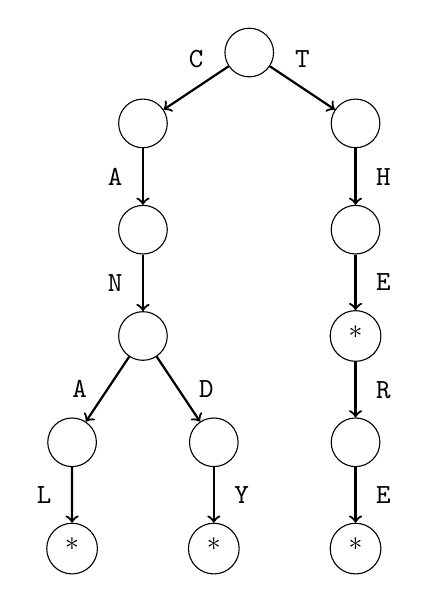
\begin{tikzpicture}[scale=0.9]
\node[draw, circle] (1) at (0,20) {$\phantom{1}$};
\node[draw, circle] (2) at (-1.5,19) {$\phantom{1}$};
\node[draw, circle] (3) at (1.5,19) {$\phantom{1}$};
\node[draw, circle] (4) at (-1.5,17.5) {$\phantom{1}$};
\node[draw, circle] (5) at (-1.5,16) {$\phantom{1}$};
\node[draw, circle] (6) at (-2.5,14.5) {$\phantom{1}$};
\node[draw, circle] (7) at (-0.5,14.5) {$\phantom{1}$};
\node[draw, circle] (8) at (-2.5,13) {*};
\node[draw, circle] (9) at (-0.5,13) {*};
\node[draw, circle] (10) at (1.5,17.5) {$\phantom{1}$};
\node[draw, circle] (11) at (1.5,16) {*};
\node[draw, circle] (12) at (1.5,14.5) {$\phantom{1}$};
\node[draw, circle] (13) at (1.5,13) {*};

\path[draw,thick,->] (1) -- node[font=\small,label=\texttt{C}] {} (2);
\path[draw,thick,->] (1) -- node[font=\small,label=\texttt{T}] {} (3);
\path[draw,thick,->] (2) -- node[font=\small,label=left:\texttt{A}] {} (4);
\path[draw,thick,->] (4) -- node[font=\small,label=left:\texttt{N}] {} (5);
\path[draw,thick,->] (5) -- node[font=\small,label=left:\texttt{A}] {} (6);
\path[draw,thick,->] (5) -- node[font=\small,label=right:\texttt{D}] {} (7);
\path[draw,thick,->] (6) -- node[font=\small,label=left:\texttt{L}] {}(8);
\path[draw,thick,->] (7) -- node[font=\small,label=right:\texttt{Y}] {} (9);
\path[draw,thick,->] (3) -- node[font=\small,label=right:\texttt{H}] {} (10);
\path[draw,thick,->] (10) -- node[font=\small,label=right:\texttt{E}] {} (11);
\path[draw,thick,->] (11) -- node[font=\small,label=right:\texttt{R}] {} (12);
\path[draw,thick,->] (12) -- node[font=\small,label=right:\texttt{E}] {} (13);
\end{tikzpicture}
\end{center}

این درخت ترای متناظر با مجموعه
$\{\texttt{CANAL},\texttt{CANDY},\texttt{THE},\texttt{THERE}\}$
است.
نویسه * در یک گره نشان می‌دهد که
یک رشته از مجموعه در آن گره پایان یافته است.
چنین نویسه‌ای لازم است، زیرا یک رشته
ممکن است پیشوندی از رشته دیگر باشد.
برای نمونه، در درخت ترای بالا، \texttt{THE}
پیشوندی از \texttt{THERE} است.

می‌توان در زمان $O(n)$ بررسی کرد که آیا ترای
شامل رشته‌ای به طول $n$ است یا خیر،
زیرا می‌توان زنجیره‌ای را که از گره ریشه آغاز می‌شود پیمایش کرد.
همچنین می‌توان رشته‌ای به طول $n$ را در زمان $O(n)$ به ترای اضافه کرد؛
نخست با پیمایش زنجیره
و سپس در صورت لزوم، افزودن گره‌های جدید به ترای.

با استفاده از ترای، می‌توان طولانی‌ترین پیشوند
از یک رشته داده‌شده را یافت
به‌طوری که آن پیشوند متعلق به مجموعه باشد.
افزون بر این، با ذخیره اطلاعات اضافه
در هر گره،
می‌توان تعداد رشته‌هایی را که به مجموعه تعلق دارند
و رشته داده‌شده پیشوند آن‌هاست محاسبه کرد.

یک ترای را می‌توان در یک آرایه ذخیره کرد:
\begin{lstlisting}
int trie[N][A];
\end{lstlisting}
که در آن $N$ حداکثر تعداد گره‌ها
(حداکثر مجموع طول رشته‌های موجود در مجموعه)
و $A$ اندازه الفبا است.
گره‌های ترای از
$0,1,2,\ldots$ شماره‌گذاری می‌شوند به طوری که شماره ریشه 0 است،
و $\texttt{trie}[s][c]$ گره بعدی در زنجیره است
هنگامی که از گره $s$ با استفاده از نویسه $c$ حرکت می‌کنیم.

\section{هشینگ رشته}

\index{hashing}
\index{string hashing}

\key{هشینگ رشته} روشی است که
امکان بررسی کارآمد برابری دو رشته را
فراهم می‌کند\footnote{این روش
توسط الگوریتم تطابق الگوی کارپ-رابین محبوبیت یافت \cite{kar87}.}.
ایده در هشینگ رشته، مقایسه مقادیر هش
رشته‌ها به جای مقایسه تک‌تک نویسه‌های آن‌ها است.

\subsubsection*{محاسبه مقادیر هش}

\index{hash value}
\index{polynomial hashing}

\key{مقدار هش} یک رشته،
عددی است که از روی نویسه‌های
آن رشته محاسبه می‌شود.
اگر دو رشته یکسان باشند،
مقادیر هش آن‌ها نیز یکسان است؛
این ویژگی امکان مقایسه رشته‌ها
بر پایه مقادیر هش آن‌ها را فراهم می‌کند.

روش متداول برای پیاده‌سازی هشینگ رشته،
\key{هشینگ چندجمله‌ای} است؛ یعنی
مقدار هش رشته \texttt{s}
به طول $n$ برابر است با:
\[(\texttt{s}[0] A^{n-1} + \texttt{s}[1] A^{n-2} + \cdots + \texttt{s}[n-1] A^0) \bmod B  ,\]
که در آن $s[0],s[1],\ldots,s[n-1]$
به عنوان کد نویسه‌های \texttt{s} در نظر گرفته می‌شوند،
و $A$ و $B$ ثابت‌های از پیش انتخاب‌شده هستند.

برای نمونه، کدهای نویسه‌های
\texttt{ALLEY} عبارتند از:
\begin{center}
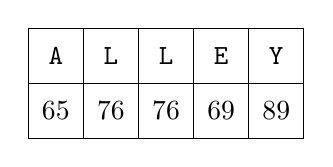
\begin{tikzpicture}[scale=0.7]
\draw (0,0) grid (5,2);

\node at (0.5, 1.5) {\texttt{A}};
\node at (1.5, 1.5) {\texttt{L}};
\node at (2.5, 1.5) {\texttt{L}};
\node at (3.5, 1.5) {\texttt{E}};
\node at (4.5, 1.5) {\texttt{Y}};

\node at (0.5, 0.5) {65};
\node at (1.5, 0.5) {76};
\node at (2.5, 0.5) {76};
\node at (3.5, 0.5) {69};
\node at (4.5, 0.5) {89};

\end{tikzpicture}
\end{center}

بنابراین، اگر $A=3$ و $B=97$ باشد، مقدار هش
\texttt{ALLEY} برابر است با:
\[(65 \cdot 3^4 + 76 \cdot 3^3 + 76 \cdot 3^2 + 69 \cdot 3^1 + 89 \cdot 3^0) \bmod 97 = 52.\]

\subsubsection*{پیش‌پردازش}

با استفاده از هش چندجمله‌ای، می‌توان مقدار هش هر زیررشته از یک رشتهٔ \texttt{s} را پس از یک پیش‌پردازش با زمان $O(n)$، در زمان $O(1)$ محاسبه کرد.
ایده این است که آرایهٔ \texttt{h} به گونه‌ای ساخته شود که
$\texttt{h}[k]$ حاوی مقدار هش پیشوند $\texttt{s}[0 \ldots k]$ باشد.
مقادیر این آرایه را می‌توان به‌صورت بازگشتی مطابق زیر محاسبه کرد:
\[
\begin{array}{lcl}
\texttt{h}[0] & = & \texttt{s}[0] \\
\texttt{h}[k] & = & (\texttt{h}[k-1] A + \texttt{s}[k]) \bmod B \\
\end{array}
\]
علاوه بر این، آرایهٔ $\texttt{p}$ را می‌سازیم
که در آن $\texttt{p}[k]=A^k \bmod B$ است:
\[
\begin{array}{lcl}
\texttt{p}[0] & = & 1 \\
\texttt{p}[k] & = & (\texttt{p}[k-1] A) \bmod B. \\
\end{array}
\]
ساخت این آرایه‌ها به زمان $O(n)$ نیاز دارد.
پس از آن، مقدار هش هر زیررشتهٔ
$\texttt{s}[a \ldots b]$
با فرض $a>0$ می‌تواند در زمان $O(1)$ با استفاده از فرمول زیر محاسبه شود:
\[(\texttt{h}[b]-\texttt{h}[a-1] \texttt{p}[b-a+1]) \bmod B\]
اگر $a=0$ باشد، مقدار هش همان $\texttt{h}[b]$ خواهد بود.

\subsubsection*{استفاده از مقادیر هش}

می‌توان رشته‌ها را با استفاده از مقادیر هش به شکلی کارا مقایسه کرد.
به‌جای مقایسهٔ تک‌تک نویسه‌های رشته‌ها،
ایده این است که مقادیر هش آن‌ها مقایسه شود.
اگر مقادیر هش برابر باشند،
رشته‌ها \emph{احتمالاً} برابرند،
و اگر مقادیر هش متفاوت باشند،
رشته‌ها \emph{قطعاً} متفاوت هستند.

با استفاده از هشینگ، اغلب می‌توان یک الگوریتم جستجوی کامل (brute force) را کارا کرد.
به عنوان مثال، مسئلهٔ تطابق الگو را در نظر بگیرید:
به ازای یک رشتهٔ $s$ و یک الگو $p$،
موقعیت‌هایی را بیابید که $p$ در $s$ رخ می‌دهد.
یک الگوریتم جستجوی کامل تمام موقعیت‌هایی را که $p$ ممکن است در آن‌ها رخ دهد پیمایش کرده و رشته‌ها را نویسه‌به‌نویسه مقایسه می‌کند.
پیچیدگی زمانی چنین الگوریتمی $O(n^2)$ است.

می‌توان با استفاده از هشینگ، الگوریتم جستجوی کامل را کاراتر کرد، زیرا این الگوریتم زیررشته‌هایی از رشته‌ها را مقایسه می‌کند.
با استفاده از هشینگ، هر مقایسه تنها $O(1)$ زمان می‌برد،
زیرا فقط مقادیر هش زیررشته‌ها مقایسه می‌شوند.
این کار منجر به الگوریتمی با پیچیدگی زمانی $O(n)$ می‌شود
که بهترین پیچیدگی زمانی ممکن برای این مسئله است.

با ترکیب هشینگ و \emph{جستجوی دودویی}،
یافتن ترتیب لغت‌نگاشتی (lexicographic) دو رشته در زمان لگاریتمی نیز امکان‌پذیر است.
این کار با محاسبهٔ طول طولانی‌ترین پیشوند مشترک دو رشته با استفاده از جستجوی دودویی انجام می‌شود.
پس از یافتن طول پیشوند مشترک،
کافی است نویسهٔ بعدی پس از پیشوند را بررسی کنیم،
زیرا این نویسه ترتیب رشته‌ها را مشخص می‌کند.

\subsubsection*{تصادم‌ها و پارامترها}

\index{تصادم}

یک خطر آشکار هنگام مقایسهٔ مقادیر هش،
وقوع یک \key{تصادم} (collision) است؛ بدین معنی که دو رشته محتوای متفاوتی دارند اما مقدار هش آن‌ها یکسان است.
در این حالت، الگوریتمی که به مقادیر هش اتکا دارد نتیجه می‌گیرد که رشته‌ها برابر هستند،
اما در واقعیت این‌گونه نیست
و الگوریتم ممکن است نتایج نادرستی ارائه دهد.

برخوردها همواره ممکن هستند،
زیرا تعداد رشته‌های متمایز بیشتر از
تعداد مقادیر هش متمایز است.
با این حال، در صورت انتخاب دقیق ثوابت $A$ و $B$،
احتمال برخورد کم است.
رویکرد متداول، انتخاب ثوابت تصادفی
نزدیک به $10^9$ است، به عنوان نمونه:
\[
\begin{array}{lcl}
A & = & 911382323 \\
B & = & 972663749 \\
\end{array}
\]

با چنین ثوابتی،
هنگام محاسبه مقادیر هش می‌توان از نوع داده \texttt{long long} استفاده کرد،
زیرا حاصل‌ضرب‌های $AB$ و $BB$ در \texttt{long long} جا می‌گیرند.
اما آیا وجود حدود $10^9$ مقدار هش متمایز کافی است؟

سه سناریو کاربرد هش را در نظر بگیرید:

\textit{سناریو ۱:} رشته‌های $x$ و $y$ با یکدیگر
مقایسه می‌شوند.
با فرض هم‌احتمال بودن همه مقادیر هش،
احتمال وقوع برخورد $1/B$ است.

\textit{سناریو ۲:} رشته $x$ با رشته‌های
$y_1,y_2,\ldots,y_n$ مقایسه می‌شود.
احتمال وقوع یک یا چند برخورد برابر است با:

\[1-(1-\frac{1}{B})^n.\]

\textit{سناریو ۳:} همه جفت‌های رشته‌های $x_1,x_2,\ldots,x_n$
با یکدیگر مقایسه می‌شوند.
احتمال وقوع یک یا چند برخورد برابر است با:
\[ 1 - \frac{B \cdot (B-1) \cdot (B-2) \cdots (B-n+1)}{B^n}.\]

جدول زیر احتمال برخورد را به ازای
$n=10^6$ و مقادیر مختلف $B$ نشان می‌دهد:

\begin{center}
\begin{tabular}{rrrr}
ثابت $B$ & سناریو ۱ & سناریو ۲ & سناریو ۳ \\
\hline
$10^3$ & $0.001000$ & $1.000000$ & $1.000000$ \\
$10^6$ & $0.000001$ & $0.632121$ & $1.000000$ \\
$10^9$ & $0.000000$ & $0.001000$ & $1.000000$ \\
$10^{12}$ & $0.000000$ & $0.000000$ & $0.393469$ \\
$10^{15}$ & $0.000000$ & $0.000000$ & $0.000500$ \\
$10^{18}$ & $0.000000$ & $0.000000$ & $0.000001$ \\
\end{tabular}
\end{center}

جدول نشان می‌دهد در سناریو ۱،
هنگام $B \approx 10^9$، احتمال برخورد ناچیز است.
در سناریو ۲، برخورد ممکن است ولی
احتمال آن همچنان بسیار کم است.
با این حال در سناریو ۳ وضعیت کاملا متفاوت است:
هنگام $B \approx 10^9$ برخورد تقریبا همواره رخ می‌دهد.

\index{birthday paradox}

پدیده موجود در سناریو ۳ تحت عنوان
\key{پارادوکس روز تولد} شناخته می‌شود: اگر $n$ نفر
در یک اتاق باشند، احتمال اینکه \emph{حداقل دو نفر}
روز تولد یکسانی داشته باشند بالاست، حتی اگر $n$ بسیار کوچک باشد.
در هشینگ نیز به همین ترتیب، با مقایسه همه مقادیر هش با یکدیگر،
احتمال برابر شدن حداقل دو مقدار هش بالاست.

می‌توان با محاسبه \emph{چندین} مقدار هش با پارامترهای مختلف،
احتمال برخورد را کاهش داد.
وقوع برخورد همزمان در همه مقادیر هش بعید است.
برای نمونه، دو مقدار هش با پارامتر
$B \approx 10^9$ معادل یک مقدار هش با پارامتر
$B \approx 10^{18}$ عمل می‌کند،
که احتمال برخورد را بسیار ناچیز می‌سازد.

برخی افراد از ثوابت $B=2^{32}$ و $B=2^{64}$ استفاده می‌کنند
که کار را راحت می‌کند، زیرا محاسبات با اعداد صحیح ۳۲ و ۶۴ بیتی
به پیمانه $2^{32}$ و $2^{64}$ انجام می‌شود.
با این حال، این انتخاب \emph{خوبی} نیست، زیرا می‌توان
ورودی‌هایی ساخت که با ثوابت به فرم $2^x$ همیشه برخورد هش ایجاد کنند \cite{pac13}.

\section{الگوریتم Z}

\index{الگوریتم Z}
\index{آرایه Z}

\key{آرایه Z} با نام \texttt{z} برای یک رشته \texttt{s} به طول $n$،
به ازای هر $k=0,1,\ldots,n-1$ شامل طول طولانی‌ترین زیررشته‌ای از \texttt{s} است
که از مکان $k$ شروع می‌شود و پیشوندی از \texttt{s} است.
بنابراین، $\texttt{z}[k]=p$ نشان می‌دهد که
$\texttt{s}[0 \ldots p-1]$ برابر با $\texttt{s}[k \ldots k+p-1]$ است.
مسائل متعددی در پردازش رشته‌ها را می‌توان با استفاده از آرایه Z به طور کارآمد حل کرد.

به عنوان مثال، آرایه Z رشته
\texttt{ACBACDACBACBACDA} به صورت زیر است:

\begin{center}
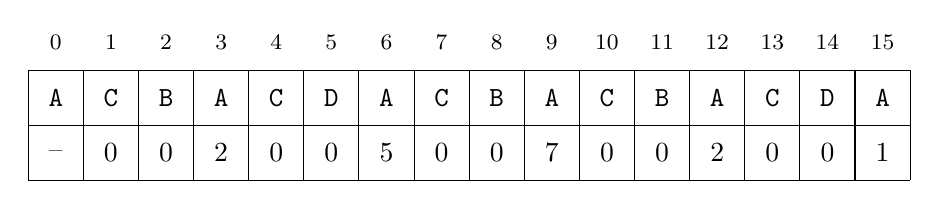
\begin{tikzpicture}[scale=0.7]
\draw (0,0) grid (16,2);

\node at (0.5, 1.5) {\texttt{A}};
\node at (1.5, 1.5) {\texttt{C}};
\node at (2.5, 1.5) {\texttt{B}};
\node at (3.5, 1.5) {\texttt{A}};
\node at (4.5, 1.5) {\texttt{C}};
\node at (5.5, 1.5) {\texttt{D}};
\node at (6.5, 1.5) {\texttt{A}};
\node at (7.5, 1.5) {\texttt{C}};
\node at (8.5, 1.5) {\texttt{B}};
\node at (9.5, 1.5) {\texttt{A}};
\node at (10.5, 1.5) {\texttt{C}};
\node at (11.5, 1.5) {\texttt{B}};
\node at (12.5, 1.5) {\texttt{A}};
\node at (13.5, 1.5) {\texttt{C}};
\node at (14.5, 1.5) {\texttt{D}};
\node at (15.5, 1.5) {\texttt{A}};

\node at (0.5, 0.5) {--};
\node at (1.5, 0.5) {0};
\node at (2.5, 0.5) {0};
\node at (3.5, 0.5) {2};
\node at (4.5, 0.5) {0};
\node at (5.5, 0.5) {0};
\node at (6.5, 0.5) {5};
\node at (7.5, 0.5) {0};
\node at (8.5, 0.5) {0};
\node at (9.5, 0.5) {7};
\node at (10.5, 0.5) {0};
\node at (11.5, 0.5) {0};
\node at (12.5, 0.5) {2};
\node at (13.5, 0.5) {0};
\node at (14.5, 0.5) {0};
\node at (15.5, 0.5) {1};

\footnotesize
\node at (0.5, 2.5) {0};
\node at (1.5, 2.5) {1};
\node at (2.5, 2.5) {2};
\node at (3.5, 2.5) {3};
\node at (4.5, 2.5) {4};
\node at (5.5, 2.5) {5};
\node at (6.5, 2.5) {6};
\node at (7.5, 2.5) {7};
\node at (8.5, 2.5) {8};
\node at (9.5, 2.5) {9};
\node at (10.5, 2.5) {10};
\node at (11.5, 2.5) {11};
\node at (12.5, 2.5) {12};
\node at (13.5, 2.5) {13};
\node at (14.5, 2.5) {14};
\node at (15.5, 2.5) {15};

\end{tikzpicture}
\end{center}

در این مورد، برای مثال $\texttt{z}[6]=5$ است،
زیرا زیررشته \texttt{ACBAC} با طول ۵
پیشوندی از \texttt{s} است،
اما زیررشته \texttt{ACBACB} با طول ۶
پیشوندی از \texttt{s} نیست.

\subsubsection*{شرح الگوریتم}

در ادامه الگوریتمی موسوم به \key{الگوریتم زد}\footnote{الگوریتم Z در \cite{gus97} به عنوان ساده‌ترین روش شناخته‌شده برای تطابق الگو در زمان خطی معرفی شد و ایده اصلی آن به \cite{mai84} نسبت داده شده است.} را شرح می‌دهیم که آرایه زد را به شکل کارآمد در زمان $O(n)$ می‌سازد.
این الگوریتم مقادیر آرایه زد را از چپ به راست محاسبه می‌کند؛ هم با استفاده از اطلاعاتی که از قبل در آرایه زد ذخیره شده‌اند و هم از طریق مقایسه کاراکتر به کاراکتر زیررشته‌ها.

برای محاسبه بهینه مقادیر آرایه زد، الگوریتم بازه‌ای مانند $[x,y]$ را نگهداری می‌کند به طوری که $\texttt{s}[x \ldots y]$ پیشوندی از \texttt{s} باشد و $y$ تا حد امکان بزرگ باشد.
از آنجا که می‌دانیم $\texttt{s}[0 \ldots y-x]$ و $\texttt{s}[x \ldots y]$ برابر هستند، می‌توانیم هنگام محاسبه مقادیر زد برای موقعیت‌های $x+1,x+2,\ldots,y$ از این اطلاعات بهره ببریم.

در هر موقعیت $k$، ابتدا مقدار $\texttt{z}[k-x]$ را بررسی می‌کنیم.
اگر $k+\texttt{z}[k-x]<y$ باشد، می‌دانیم که $\texttt{z}[k]=\texttt{z}[k-x]$ است.
اما اگر $k+\texttt{z}[k-x] \ge y$ باشد، $\texttt{s}[0 \ldots y-k]$ برابر با $\texttt{s}[k \ldots y]$ است، و برای تعیین مقدار $\texttt{z}[k]$ باید زیررشته‌ها را کاراکتر به کاراکتر مقایسه کنیم.
با این وجود، الگوریتم همچنان در زمان $O(n)$ اجرا می‌شود، زیرا مقایسه را از موقعیت‌های $y-k+1$ و $y+1$ آغاز می‌کنیم.

به عنوان مثال، فرض کنید می‌خواهیم آرایه زد زیر را بسازیم:

\begin{center}
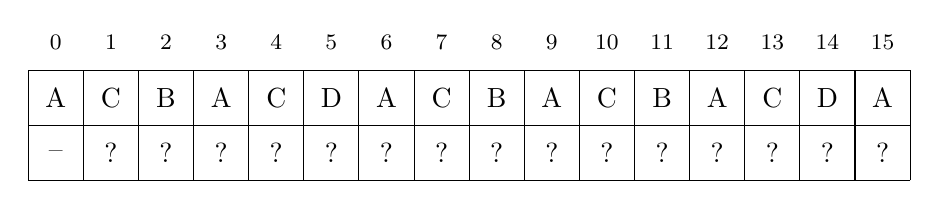
\begin{tikzpicture}[scale=0.7]
\draw (0,0) grid (16,2);

\node at (0.5, 1.5) {A};
\node at (1.5, 1.5) {C};
\node at (2.5, 1.5) {B};
\node at (3.5, 1.5) {A};
\node at (4.5, 1.5) {C};
\node at (5.5, 1.5) {D};
\node at (6.5, 1.5) {A};
\node at (7.5, 1.5) {C};
\node at (8.5, 1.5) {B};
\node at (9.5, 1.5) {A};
\node at (10.5, 1.5) {C};
\node at (11.5, 1.5) {B};
\node at (12.5, 1.5) {A};
\node at (13.5, 1.5) {C};
\node at (14.5, 1.5) {D};
\node at (15.5, 1.5) {A};

\node at (0.5, 0.5) {--};
\node at (1.5, 0.5) {?};
\node at (2.5, 0.5) {?};
\node at (3.5, 0.5) {?};
\node at (4.5, 0.5) {?};
\node at (5.5, 0.5) {?};
\node at (6.5, 0.5) {?};
\node at (7.5, 0.5) {?};
\node at (8.5, 0.5) {?};
\node at (9.5, 0.5) {?};
\node at (10.5, 0.5) {?};
\node at (11.5, 0.5) {?};
\node at (12.5, 0.5) {?};
\node at (13.5, 0.5) {?};
\node at (14.5, 0.5) {?};
\node at (15.5, 0.5) {?};

\footnotesize
\node at (0.5, 2.5) {0};
\node at (1.5, 2.5) {1};
\node at (2.5, 2.5) {2};
\node at (3.5, 2.5) {3};
\node at (4.5, 2.5) {4};
\node at (5.5, 2.5) {5};
\node at (6.5, 2.5) {6};
\node at (7.5, 2.5) {7};
\node at (8.5, 2.5) {8};
\node at (9.5, 2.5) {9};
\node at (10.5, 2.5) {10};
\node at (11.5, 2.5) {11};
\node at (12.5, 2.5) {12};
\node at (13.5, 2.5) {13};
\node at (14.5, 2.5) {14};
\node at (15.5, 2.5) {15};

\end{tikzpicture}
\end{center}

پس از محاسبه مقدار $\texttt{z}[6]=5$، بازه فعلی $[x,y]$ برابر با $[6,10]$ خواهد بود:

\begin{center}
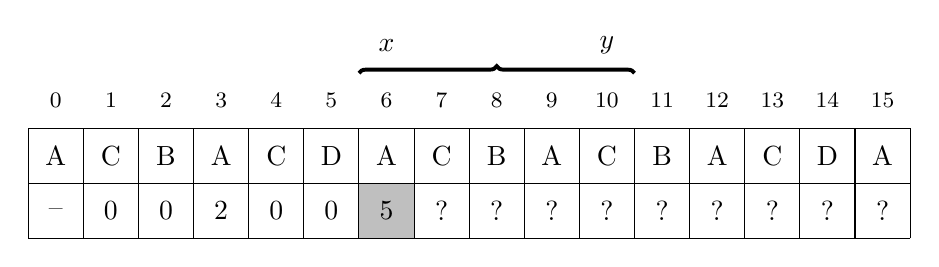
\begin{tikzpicture}[scale=0.7]
\fill[color=lightgray] (6,0) rectangle (7,1);
\draw (0,0) grid (16,2);

\node at (0.5, 1.5) {A};
\node at (1.5, 1.5) {C};
\node at (2.5, 1.5) {B};
\node at (3.5, 1.5) {A};
\node at (4.5, 1.5) {C};
\node at (5.5, 1.5) {D};
\node at (6.5, 1.5) {A};
\node at (7.5, 1.5) {C};
\node at (8.5, 1.5) {B};
\node at (9.5, 1.5) {A};
\node at (10.5, 1.5) {C};
\node at (11.5, 1.5) {B};
\node at (12.5, 1.5) {A};
\node at (13.5, 1.5) {C};
\node at (14.5, 1.5) {D};
\node at (15.5, 1.5) {A};

\node at (0.5, 0.5) {--};
\node at (1.5, 0.5) {0};
\node at (2.5, 0.5) {0};
\node at (3.5, 0.5) {2};
\node at (4.5, 0.5) {0};
\node at (5.5, 0.5) {0};
\node at (6.5, 0.5) {5};
\node at (7.5, 0.5) {?};
\node at (8.5, 0.5) {?};
\node at (9.5, 0.5) {?};
\node at (10.5, 0.5) {?};
\node at (11.5, 0.5) {?};
\node at (12.5, 0.5) {?};
\node at (13.5, 0.5) {?};
\node at (14.5, 0.5) {?};
\node at (15.5, 0.5) {?};

\draw [decoration={brace}, decorate, line width=0.5mm] (6,3.00) -- (11,3.00);

\node at (6.5,3.50) {$x$};
\node at (10.5,3.50) {$y$};


\footnotesize
\node at (0.5, 2.5) {0};
\node at (1.5, 2.5) {1};
\node at (2.5, 2.5) {2};
\node at (3.5, 2.5) {3};
\node at (4.5, 2.5) {4};
\node at (5.5, 2.5) {5};
\node at (6.5, 2.5) {6};
\node at (7.5, 2.5) {7};
\node at (8.5, 2.5) {8};
\node at (9.5, 2.5) {9};
\node at (10.5, 2.5) {10};
\node at (11.5, 2.5) {11};
\node at (12.5, 2.5) {12};
\node at (13.5, 2.5) {13};
\node at (14.5, 2.5) {14};
\node at (15.5, 2.5) {15};

\end{tikzpicture}
\end{center}

اکنون می‌توان مقادیر بعدی آرایه $Z$ را به شکل کارآمد محاسبه کرد، زیرا می‌دانیم $\texttt{s}[0 \ldots 4]$ و $\texttt{s}[6 \ldots 10]$ برابرند. نخست، چون $\texttt{z}[1] = \texttt{z}[2] = 0$ است، بلافاصله نتیجه می‌شود $\texttt{z}[7] = \texttt{z}[8] = 0$:

\begin{center}
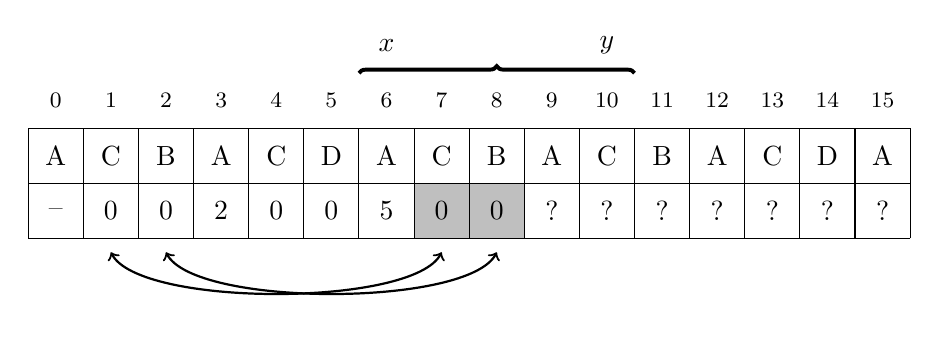
\begin{tikzpicture}[scale=0.7]
\fill[color=lightgray] (7,0) rectangle (9,1);
\draw (0,0) grid (16,2);

\node at (0.5, 1.5) {A};
\node at (1.5, 1.5) {C};
\node at (2.5, 1.5) {B};
\node at (3.5, 1.5) {A};
\node at (4.5, 1.5) {C};
\node at (5.5, 1.5) {D};
\node at (6.5, 1.5) {A};
\node at (7.5, 1.5) {C};
\node at (8.5, 1.5) {B};
\node at (9.5, 1.5) {A};
\node at (10.5, 1.5) {C};
\node at (11.5, 1.5) {B};
\node at (12.5, 1.5) {A};
\node at (13.5, 1.5) {C};
\node at (14.5, 1.5) {D};
\node at (15.5, 1.5) {A};

\node at (0.5, 0.5) {--};
\node at (1.5, 0.5) {0};
\node at (2.5, 0.5) {0};
\node at (3.5, 0.5) {2};
\node at (4.5, 0.5) {0};
\node at (5.5, 0.5) {0};
\node at (6.5, 0.5) {5};
\node at (7.5, 0.5) {0};
\node at (8.5, 0.5) {0};
\node at (9.5, 0.5) {?};
\node at (10.5, 0.5) {?};
\node at (11.5, 0.5) {?};
\node at (12.5, 0.5) {?};
\node at (13.5, 0.5) {?};
\node at (14.5, 0.5) {?};
\node at (15.5, 0.5) {?};


\draw [decoration={brace}, decorate, line width=0.5mm] (6,3.00) -- (11,3.00);

\node at (6.5,3.50) {$x$};
\node at (10.5,3.50) {$y$};

\footnotesize
\node at (0.5, 2.5) {0};
\node at (1.5, 2.5) {1};
\node at (2.5, 2.5) {2};
\node at (3.5, 2.5) {3};
\node at (4.5, 2.5) {4};
\node at (5.5, 2.5) {5};
\node at (6.5, 2.5) {6};
\node at (7.5, 2.5) {7};
\node at (8.5, 2.5) {8};
\node at (9.5, 2.5) {9};
\node at (10.5, 2.5) {10};
\node at (11.5, 2.5) {11};
\node at (12.5, 2.5) {12};
\node at (13.5, 2.5) {13};
\node at (14.5, 2.5) {14};
\node at (15.5, 2.5) {15};


\draw[thick,<->] (7.5,-0.25) .. controls (7,-1.25) and (2,-1.25) .. (1.5,-0.25);
\draw[thick,<->] (8.5,-0.25) .. controls (8,-1.25) and (3,-1.25) .. (2.5,-0.25);
\end{tikzpicture}
\end{center}

سپس، چون $\texttt{z}[3]=2$ است، می‌دانیم $\texttt{z}[9] \ge 2$:

\begin{center}
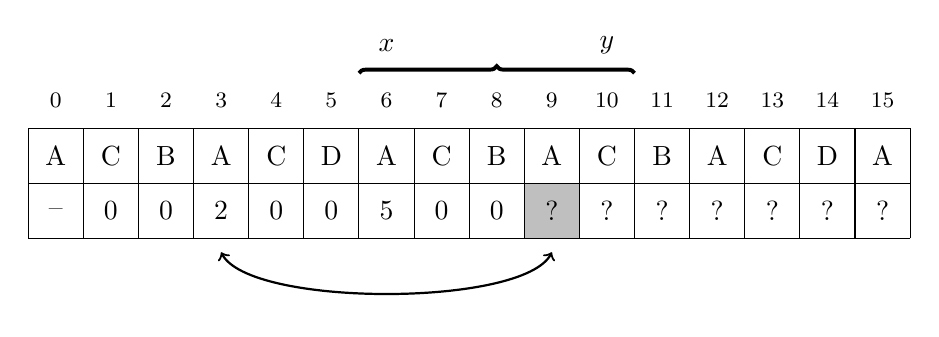
\begin{tikzpicture}[scale=0.7]
\fill[color=lightgray] (9,0) rectangle (10,1);
\draw (0,0) grid (16,2);

\node at (0.5, 1.5) {A};
\node at (1.5, 1.5) {C};
\node at (2.5, 1.5) {B};
\node at (3.5, 1.5) {A};
\node at (4.5, 1.5) {C};
\node at (5.5, 1.5) {D};
\node at (6.5, 1.5) {A};
\node at (7.5, 1.5) {C};
\node at (8.5, 1.5) {B};
\node at (9.5, 1.5) {A};
\node at (10.5, 1.5) {C};
\node at (11.5, 1.5) {B};
\node at (12.5, 1.5) {A};
\node at (13.5, 1.5) {C};
\node at (14.5, 1.5) {D};
\node at (15.5, 1.5) {A};

\node at (0.5, 0.5) {--};
\node at (1.5, 0.5) {0};
\node at (2.5, 0.5) {0};
\node at (3.5, 0.5) {2};
\node at (4.5, 0.5) {0};
\node at (5.5, 0.5) {0};
\node at (6.5, 0.5) {5};
\node at (7.5, 0.5) {0};
\node at (8.5, 0.5) {0};
\node at (9.5, 0.5) {?};
\node at (10.5, 0.5) {?};
\node at (11.5, 0.5) {?};
\node at (12.5, 0.5) {?};
\node at (13.5, 0.5) {?};
\node at (14.5, 0.5) {?};
\node at (15.5, 0.5) {?};

\draw [decoration={brace}, decorate, line width=0.5mm] (6,3.00) -- (11,3.00);

\node at (6.5,3.50) {$x$};
\node at (10.5,3.50) {$y$};


\footnotesize
\node at (0.5, 2.5) {0};
\node at (1.5, 2.5) {1};
\node at (2.5, 2.5) {2};
\node at (3.5, 2.5) {3};
\node at (4.5, 2.5) {4};
\node at (5.5, 2.5) {5};
\node at (6.5, 2.5) {6};
\node at (7.5, 2.5) {7};
\node at (8.5, 2.5) {8};
\node at (9.5, 2.5) {9};
\node at (10.5, 2.5) {10};
\node at (11.5, 2.5) {11};
\node at (12.5, 2.5) {12};
\node at (13.5, 2.5) {13};
\node at (14.5, 2.5) {14};
\node at (15.5, 2.5) {15};

\draw[thick,<->] (9.5,-0.25) .. controls (9,-1.25) and (4,-1.25) .. (3.5,-0.25);
\end{tikzpicture}
\end{center}

با این حال، اطلاعی از رشته بعد از موقعیت 10 نداریم؛ باید زیررشته‌ها نویسه‌به‌نویسه مقایسه شوند:

\begin{center}
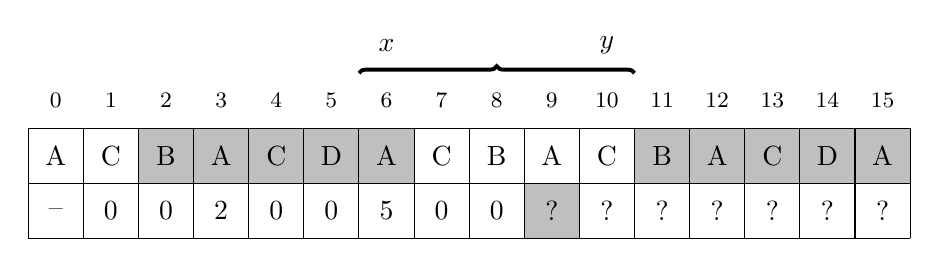
\begin{tikzpicture}[scale=0.7]
\fill[color=lightgray] (9,0) rectangle (10,1);
\fill[color=lightgray] (2,1) rectangle (7,2);
\fill[color=lightgray] (11,1) rectangle (16,2);


\draw (0,0) grid (16,2);

\node at (0.5, 1.5) {A};
\node at (1.5, 1.5) {C};
\node at (2.5, 1.5) {B};
\node at (3.5, 1.5) {A};
\node at (4.5, 1.5) {C};
\node at (5.5, 1.5) {D};
\node at (6.5, 1.5) {A};
\node at (7.5, 1.5) {C};
\node at (8.5, 1.5) {B};
\node at (9.5, 1.5) {A};
\node at (10.5, 1.5) {C};
\node at (11.5, 1.5) {B};
\node at (12.5, 1.5) {A};
\node at (13.5, 1.5) {C};
\node at (14.5, 1.5) {D};
\node at (15.5, 1.5) {A};

\node at (0.5, 0.5) {--};
\node at (1.5, 0.5) {0};
\node at (2.5, 0.5) {0};
\node at (3.5, 0.5) {2};
\node at (4.5, 0.5) {0};
\node at (5.5, 0.5) {0};
\node at (6.5, 0.5) {5};
\node at (7.5, 0.5) {0};
\node at (8.5, 0.5) {0};
\node at (9.5, 0.5) {?};
\node at (10.5, 0.5) {?};
\node at (11.5, 0.5) {?};
\node at (12.5, 0.5) {?};
\node at (13.5, 0.5) {?};
\node at (14.5, 0.5) {?};
\node at (15.5, 0.5) {?};

\draw [decoration={brace}, decorate, line width=0.5mm] (6,3.00) -- (11,3.00);

\node at (6.5,3.50) {$x$};
\node at (10.5,3.50) {$y$};


\footnotesize
\node at (0.5, 2.5) {0};
\node at (1.5, 2.5) {1};
\node at (2.5, 2.5) {2};
\node at (3.5, 2.5) {3};
\node at (4.5, 2.5) {4};
\node at (5.5, 2.5) {5};
\node at (6.5, 2.5) {6};
\node at (7.5, 2.5) {7};
\node at (8.5, 2.5) {8};
\node at (9.5, 2.5) {9};
\node at (10.5, 2.5) {10};
\node at (11.5, 2.5) {11};
\node at (12.5, 2.5) {12};
\node at (13.5, 2.5) {13};
\node at (14.5, 2.5) {14};
\node at (15.5, 2.5) {15};

%\draw[thick,<->] (11.5,-0.25) .. controls (11,-1.25) and (3,-1.25) .. (2.5,-0.25);
\end{tikzpicture}
\end{center}

مشخص می‌شود که $\texttt{z}[9]=7$ است،
بنابراین بازه جدید $[x,y]$ برابر $[9,15]$ می‌شود:

\begin{center}
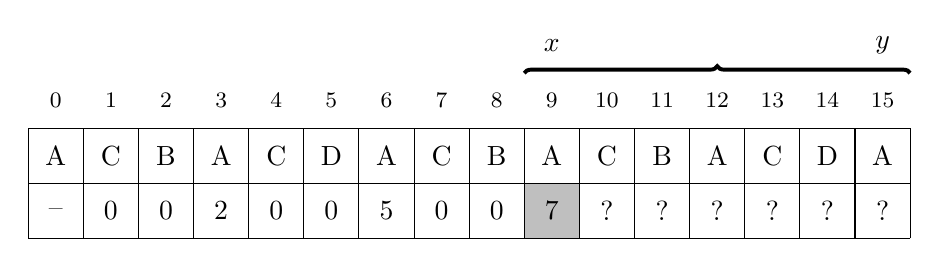
\begin{tikzpicture}[scale=0.7]
\fill[color=lightgray] (9,0) rectangle (10,1);
\draw (0,0) grid (16,2);

\node at (0.5, 1.5) {A};
\node at (1.5, 1.5) {C};
\node at (2.5, 1.5) {B};
\node at (3.5, 1.5) {A};
\node at (4.5, 1.5) {C};
\node at (5.5, 1.5) {D};
\node at (6.5, 1.5) {A};
\node at (7.5, 1.5) {C};
\node at (8.5, 1.5) {B};
\node at (9.5, 1.5) {A};
\node at (10.5, 1.5) {C};
\node at (11.5, 1.5) {B};
\node at (12.5, 1.5) {A};
\node at (13.5, 1.5) {C};
\node at (14.5, 1.5) {D};
\node at (15.5, 1.5) {A};

\node at (0.5, 0.5) {--};
\node at (1.5, 0.5) {0};
\node at (2.5, 0.5) {0};
\node at (3.5, 0.5) {2};
\node at (4.5, 0.5) {0};
\node at (5.5, 0.5) {0};
\node at (6.5, 0.5) {5};
\node at (7.5, 0.5) {0};
\node at (8.5, 0.5) {0};
\node at (9.5, 0.5) {7};
\node at (10.5, 0.5) {?};
\node at (11.5, 0.5) {?};
\node at (12.5, 0.5) {?};
\node at (13.5, 0.5) {?};
\node at (14.5, 0.5) {?};
\node at (15.5, 0.5) {?};

\draw [decoration={brace}, decorate, line width=0.5mm] (9,3.00) -- (16,3.00);

\node at (9.5,3.50) {$x$};
\node at (15.5,3.50) {$y$};

\footnotesize
\node at (0.5, 2.5) {0};
\node at (1.5, 2.5) {1};
\node at (2.5, 2.5) {2};
\node at (3.5, 2.5) {3};
\node at (4.5, 2.5) {4};
\node at (5.5, 2.5) {5};
\node at (6.5, 2.5) {6};
\node at (7.5, 2.5) {7};
\node at (8.5, 2.5) {8};
\node at (9.5, 2.5) {9};
\node at (10.5, 2.5) {10};
\node at (11.5, 2.5) {11};
\node at (12.5, 2.5) {12};
\node at (13.5, 2.5) {13};
\node at (14.5, 2.5) {14};
\node at (15.5, 2.5) {15};

% \draw[thick,<->] (9.5,-0.25) .. controls (9,-1.25) and (4,-1.25) .. (3.5,-0.25);
\end{tikzpicture}
\end{center}

پس از این، تمام مقادیر باقی‌مانده آرایه Z را می‌توان با استفاده از اطلاعاتی که تاکنون درون آرایه Z ذخیره شده است، تعیین کرد:

\begin{center}
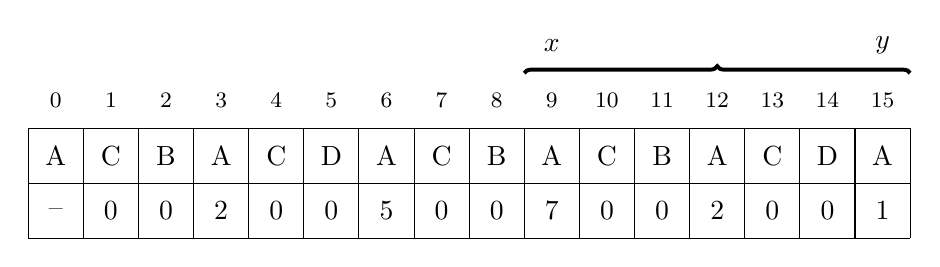
\begin{tikzpicture}[scale=0.7]
\draw (0,0) grid (16,2);

\node at (0.5, 1.5) {A};
\node at (1.5, 1.5) {C};
\node at (2.5, 1.5) {B};
\node at (3.5, 1.5) {A};
\node at (4.5, 1.5) {C};
\node at (5.5, 1.5) {D};
\node at (6.5, 1.5) {A};
\node at (7.5, 1.5) {C};
\node at (8.5, 1.5) {B};
\node at (9.5, 1.5) {A};
\node at (10.5, 1.5) {C};
\node at (11.5, 1.5) {B};
\node at (12.5, 1.5) {A};
\node at (13.5, 1.5) {C};
\node at (14.5, 1.5) {D};
\node at (15.5, 1.5) {A};

\node at (0.5, 0.5) {--};
\node at (1.5, 0.5) {0};
\node at (2.5, 0.5) {0};
\node at (3.5, 0.5) {2};
\node at (4.5, 0.5) {0};
\node at (5.5, 0.5) {0};
\node at (6.5, 0.5) {5};
\node at (7.5, 0.5) {0};
\node at (8.5, 0.5) {0};
\node at (9.5, 0.5) {7};
\node at (10.5, 0.5) {0};
\node at (11.5, 0.5) {0};
\node at (12.5, 0.5) {2};
\node at (13.5, 0.5) {0};
\node at (14.5, 0.5) {0};
\node at (15.5, 0.5) {1};

\draw [decoration={brace}, decorate, line width=0.5mm] (9,3.00) -- (16,3.00);

\node at (9.5,3.50) {$x$};
\node at (15.5,3.50) {$y$};


\footnotesize
\node at (0.5, 2.5) {0};
\node at (1.5, 2.5) {1};
\node at (2.5, 2.5) {2};
\node at (3.5, 2.5) {3};
\node at (4.5, 2.5) {4};
\node at (5.5, 2.5) {5};
\node at (6.5, 2.5) {6};
\node at (7.5, 2.5) {7};
\node at (8.5, 2.5) {8};
\node at (9.5, 2.5) {9};
\node at (10.5, 2.5) {10};
\node at (11.5, 2.5) {11};
\node at (12.5, 2.5) {12};
\node at (13.5, 2.5) {13};
\node at (14.5, 2.5) {14};
\node at (15.5, 2.5) {15};

\end{tikzpicture}
\end{center}

\subsubsection{استفاده از آرایه Z}

انتخاب بین درهم‌سازی رشته یا الگوریتم Z اغلب سلیقه‌ای است.
برخلاف درهم‌سازی، الگوریتم Z همواره کار می‌کند و خطر تصادم ندارد.
از طرف دیگر، پیاده‌سازی الگوریتم Z دشوارتر است و برخی مسائل فقط با درهم‌سازی حل می‌شوند.

به عنوان مثال، مسئله تطابق الگو را دوباره در نظر بگیرید که هدف در آن، یافتن رخدادهای الگوی $p$ در رشته $s$ است.
این مسئله پیش‌تر با درهم‌سازی رشته به‌طور کارا حل شد، ولی الگوریتم Z روش دیگری برای حل آن ارائه می‌دهد.

یک ایده معمول در پردازش رشته ساخت رشته‌ای متشکل از چند رشته با جداکننده نویسه خاص است. در این مسئله می‌توان رشته $p$\texttt{\#}$s$ را ساخت، جایی که $p$ و $s$ با نویسه خاص \texttt{\#} جدا می‌شوند که درون رشته‌ها نیست. آرایه Z رشته $p$\texttt{\#}$s$ موقعیت‌های وقوع $p$ در $s$ را مشخص می‌کند، زیرا این موقعیت‌ها حاوی طول $p$ هستند.

برای مثال، اگر $s=$\texttt{HATTIVATTI} و $p=$\texttt{ATT} باشد، آرایه Z بدین صورت است:

\begin{center}
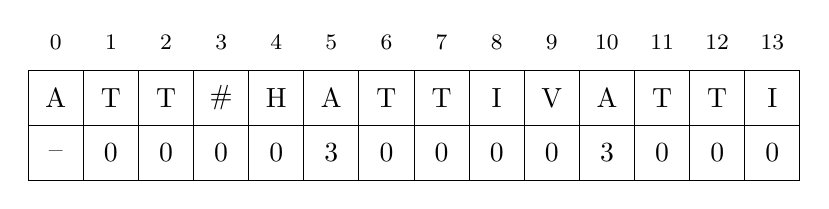
\begin{tikzpicture}[scale=0.7]
\draw (0,0) grid (14,2);

\node at (0.5, 1.5) {A};
\node at (1.5, 1.5) {T};
\node at (2.5, 1.5) {T};
\node at (3.5, 1.5) {\#};
\node at (4.5, 1.5) {H};
\node at (5.5, 1.5) {A};
\node at (6.5, 1.5) {T};
\node at (7.5, 1.5) {T};
\node at (8.5, 1.5) {I};
\node at (9.5, 1.5) {V};
\node at (10.5, 1.5) {A};
\node at (11.5, 1.5) {T};
\node at (12.5, 1.5) {T};
\node at (13.5, 1.5) {I};

\node at (0.5, 0.5) {--};
\node at (1.5, 0.5) {0};
\node at (2.5, 0.5) {0};
\node at (3.5, 0.5) {0};
\node at (4.5, 0.5) {0};
\node at (5.5, 0.5) {3};
\node at (6.5, 0.5) {0};
\node at (7.5, 0.5) {0};
\node at (8.5, 0.5) {0};
\node at (9.5, 0.5) {0};
\node at (10.5, 0.5) {3};
\node at (11.5, 0.5) {0};
\node at (12.5, 0.5) {0};
\node at (13.5, 0.5) {0};

\footnotesize
\node at (0.5, 2.5) {0};
\node at (1.5, 2.5) {1};
\node at (2.5, 2.5) {2};
\node at (3.5, 2.5) {3};
\node at (4.5, 2.5) {4};
\node at (5.5, 2.5) {5};
\node at (6.5, 2.5) {6};
\node at (7.5, 2.5) {7};
\node at (8.5, 2.5) {8};
\node at (9.5, 2.5) {9};
\node at (10.5, 2.5) {10};
\node at (11.5, 2.5) {11};
\node at (12.5, 2.5) {12};
\node at (13.5, 2.5) {13};
\end{tikzpicture}
\end{center}

موقعیت‌های 5 و 10 مقدار 3 دارند، یعنی الگوی \texttt{ATT} در موقعیت‌های متناظر \texttt{HATTIVATTI} رخ می‌دهد.

پیچیدگی زمانی الگوریتم حاصل خطی است، ساخت آرایه Z و پیمایش مقادیر آن کفایت می‌کند.

\subsubsection{پیاده‌سازی}

این پیاده‌سازی کوتاه الگوریتم Z است که بردار متناظر با آرایه Z را برمی‌گرداند.

\begin{lstlisting}
vector<int> z(string s) {
    int n = s.size();
    vector<int> z(n);
    int x = 0, y = 0;
    for (int i = 1; i < n; i++) {
        z[i] = max(0,min(z[i-x],y-i+1));
        while (i+z[i] < n && s[z[i]] == s[i+z[i]]) {
            x = i; y = i+z[i]; z[i]++;
        }
    }
    return z;
}
\end{lstlisting}